\documentclass[12pt]{article}
\usepackage[margin=1in]{geometry}
\usepackage{amsmath, amssymb}
\usepackage{fontspec}
\usepackage{bangla}
\usepackage{tikz}
\usetikzlibrary{arrows.meta, angles, quotes, 3d, calc}
\usepackage{graphicx}

% Configure Kalpurush font for Bangla rendering
\setmainfont{Kalpurush}

\title{\textbf{ভেক্টর বীজগণিত ও ক্যালকুলাস সমস্যাবালী (Vector Algebra \& Calculus Problem Set)}}
\author{STEM Educator}
\date{}

\begin{document}
\maketitle

% ----------------------------------------------------------------------
% Question 51
% ----------------------------------------------------------------------
\noindent\rule{\textwidth}{1pt}
\subsection*{প্রশ্ন ৫১ (Question 51)}

\textbf{প্রশ্ন:} ধরি, ত্রিমাত্রিক স্থানে তিনটি ভেক্টর যথাক্রমে $\vec{a} = -\hat{i} - \hat{k}$, $\vec{b} = -\hat{i} + \hat{j}$ এবং $\vec{c} = \hat{i} + 2\hat{j} + 3\hat{k}$। যদি $\vec{r}$ এমন একটি ভেক্টর হয় যা $\vec{r} \times \vec{b} = \vec{c} \times \vec{b}$ এবং $\vec{r} \cdot \vec{a} = 0$ সম্পর্ক দুটি সিদ্ধ করে, তবে $\vec{r} \cdot \vec{b}$ এর মান নির্ণয় করো। 

(Let three vectors in three-dimensional space be $\vec{a} = -\hat{i} - \hat{k}$, $\vec{b} = -\hat{i} + \hat{j}$, and $\vec{c} = \hat{i} + 2\hat{j} + 3\hat{k}$. If $\vec{r}$ is a vector satisfying $\vec{r} \times \vec{b} = \vec{c} \times \vec{b}$ and $\vec{r} \cdot \vec{a} = 0$, find the value of $\vec{r} \cdot \vec{b}$.)

\begin{center}
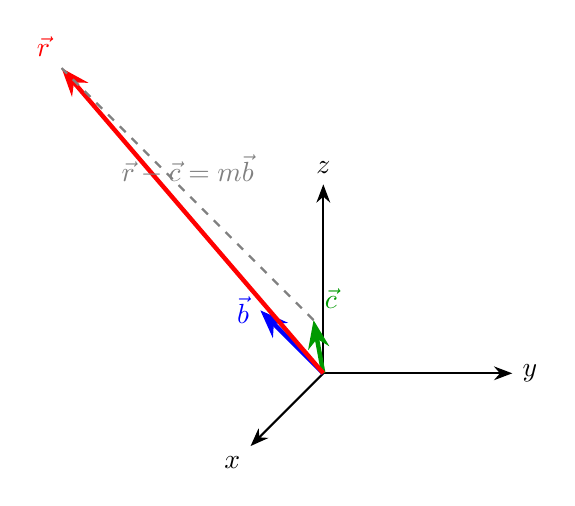
\begin{tikzpicture}[scale=0.8, >=Stealth]
  \draw[->, thick] (0,0,0) -- (3,0,0) node[right]{$y$};
  \draw[->, thick] (0,0,0) -- (0,3,0) node[above]{$z$};
  \draw[->, thick] (0,0,0) -- (0,0,3) node[below left]{$x$};
  \draw[->, blue, ultra thick] (0,0,0) -- (-1,1,0) node[left]{$\vec{b}$};
  \draw[->, green!60!black, ultra thick] (0,0,0) -- (1,2,3) node[above right]{$\vec{c}$};
  \draw[->, red, ultra thick] (0,0,0) -- (-3,6,3) node[above left]{$\vec{r}$};
  \draw[dashed, thick, gray] (1,2,3) -- (-3,6,3) node[midway, above]{$\vec{r}-\vec{c} = m\vec{b}$};
\end{tikzpicture}
\end{center}

\textbf{সমাধান:} \\
দেওয়া আছে প্রথম সম্পর্কটি:
$$\vec{r} \times \vec{b} = \vec{c} \times \vec{b} \implies (\vec{r} - \vec{c}) \times \vec{b} = \vec{0}$$
যেহেতু দুটি অশূন্য ভেক্টরের ক্রস গুণফল শূন্য এসেছে, সেহেতু ভেক্টর $(\vec{r} - \vec{c})$ এবং $\vec{b}$ পরস্পর সমান্তরাল বা সমরেখ। অতএব, আমরা লিখতে পারি:
$$\vec{r} - \vec{c} = m\vec{b} \implies \vec{r} = \vec{c} + m\vec{b} \quad \text{--- (i)} \quad \text{[যেখানে } m \text{ একটি স্কেলার রাশি]}$$
এখন সমীকরণ (i) এর উভয় পক্ষে $\vec{a}$ দ্বারা ডট গুণ করে পাই:
$$\vec{r} \cdot \vec{a} = \vec{c} \cdot \vec{a} + m(\vec{b} \cdot \vec{a})$$
শর্তানুসারে, $\vec{r} \cdot \vec{a} = 0$। অতএব:
$$0 = \vec{c} \cdot \vec{a} + m(\vec{b} \cdot \vec{a}) \implies m = -\frac{\vec{c} \cdot \vec{a}}{\vec{b} \cdot \vec{a}} \quad \text{--- (ii)}$$
প্রদত্ত ভেক্টরসমূহের ডট গুণফল হিসাব করি:
$$\vec{c} \cdot \vec{a} = (\hat{i} + 2\hat{j} + 3\hat{k}) \cdot (-\hat{i} - \hat{k}) = (1)(-1) + (2)(0) + (3)(-1) = -1 - 3 = -4$$
$$\vec{b} \cdot \vec{a} = (-\hat{i} + \hat{j}) \cdot (-\hat{i} - \hat{k}) = (-1)(-1) + (1)(0) + (0)(-1) = 1$$
সমীকরণ (ii)-এ মানগুলো বসিয়ে পাই:
$$m = -\frac{-4}{1} = 4$$
সুতরাং, সমীকরণ (i) থেকে পাই:
$$\vec{r} = \vec{c} + 4\vec{b}$$
এখন আমাদের কাঙ্ক্ষিত মান $\vec{r} \cdot \vec{b}$ নির্ণয় করি:
$$\vec{r} \cdot \vec{b} = (\vec{c} + 4\vec{b}) \cdot \vec{b} = \vec{c} \cdot \vec{b} + 4|\vec{b}|^2 \quad \text{--- (iii)}$$
এখানে:
$$\vec{c} \cdot \vec{b} = (\hat{i} + 2\hat{j} + 3\hat{k}) \cdot (-\hat{i} + \hat{j}) = (1)(-1) + (2)(1) + (3)(0) = -1 + 2 = 1$$
$$|\vec{b}|^2 = (-1)^2 + (1)^2 + 0^2 = 2$$
সমীকরণ (iii)-এ মানগুলো বসিয়ে পাই:
$$\vec{r} \cdot \vec{b} = 1 + 4(2) = 9$$
\textbf{উত্তর:} $9$

\vspace{0.8cm}

% ----------------------------------------------------------------------
% Question 52
% ----------------------------------------------------------------------
\noindent\rule{\textwidth}{1pt}
\subsection*{প্রশ্ন ৫২ (Question 52)}

\textbf{প্রশ্ন:} ধরি, ত্রিমাত্রিক কার্তেসীয় সমতলে OXY-তে একটি গতিশীল বিন্দুর অবস্থান ভেক্টর $\vec{r}$ এমনভাবে পরিবর্তিত হয় যেন এটি $\vec{r} \cdot (\vec{r} + 6\hat{j}) = 7$ সমীকরণটি সিদ্ধ করে। যদি এই সঞ্চারপথটি স্থানাঙ্ক অক্ষসমূহকে চারটি ভিন্ন বিন্দুতে ছেদ করে, তবে এই ছেদবিন্দুগুলি যোগ করে গঠিত চতুর্ভুজের ক্ষেত্রফল নির্ণয় করো। 

(Let the position vector $\vec{r}$ of a moving point in the 2D Cartesian plane OXY vary such that it satisfies $\vec{r} \cdot (\vec{r} + 6\hat{j}) = 7$. If this locus intersects the coordinate axes at four distinct points, find the area of the quadrilateral formed by joining these intersection points.)

\begin{center}
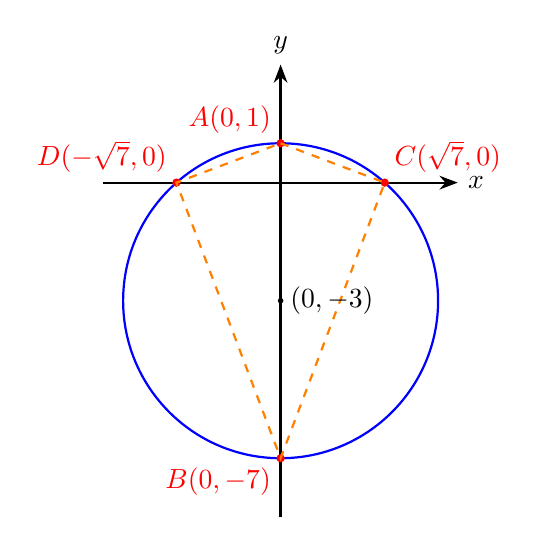
\begin{tikzpicture}[scale=0.5, >=Stealth]
  \draw[->, thick] (-4.5,0) -- (4.5,0) node[right]{$x$};
  \draw[->, thick] (0,-8.5) -- (0,3) node[above]{$y$};
  \draw[thick, blue] (0,-3) circle (4);
  \fill[red] (0,1) circle (3pt) node[above left]{$A(0,1)$};
  \fill[red] (0,-7) circle (3pt) node[below left]{$B(0,-7)$};
  \fill[red] ({sqrt(7)},0) circle (3pt) node[above right]{$C(\sqrt{7},0)$};
  \fill[red] ({-sqrt(7)},0) circle (3pt) node[above left]{$D(-\sqrt{7},0)$};
  \draw[thick, dashed, orange] (0,1) -- ({sqrt(7)},0) -- (0,-7) -- ({-sqrt(7)},0) -- cycle;
  \fill (0,-3) circle (2pt) node[right]{$(0,-3)$};
\end{tikzpicture}
\end{center}

\textbf{সমাধান:} \\
ধরি, অবস্থান ভেক্টর $\vec{r} = x\hat{i} + y\hat{j}$। \\
প্রদত্ত সমীকরণ:
$$\vec{r} \cdot (\vec{r} + 6\hat{j}) = 7$$
$$(x\hat{i} + y\hat{j}) \cdot (x\hat{i} + (y+6)\hat{j}) = 7$$
$$\Rightarrow x^2 + y(y+6) = 7 \implies x^2 + y^2 + 6y = 7$$
বৃত্তের সাধারণ সমীকরণ অনুযায়ী সাজিয়ে পাই:
$$x^2 + (y+3)^2 = 7 + 9 = 16$$
এটি একটি বৃত্তের সমীকরণ যার কেন্দ্র $(0, -3)$ এবং ব্যাসার্ধ $R = 4$।

\textbf{স্থানাঙ্ক অক্ষদ্বয়ের ছেদবিন্দুসমূহ নির্ণয়:} \\
১. $y$-অক্ষের ছেদবিন্দু (যেখানে $x = 0$):
$$0^2 + y^2 + 6y - 7 = 0 \implies (y+7)(y-1) = 0 \implies y = 1 \text{ অথবা } y = -7$$
অতএব, $y$-অক্ষের ছেদবিন্দুদ্বয় হলো: $A(0, 1)$ এবং $B(0, -7)$। \\
২. $x$-অক্ষের ছেদবিন্দু (যেখানে $y = 0$):
$$x^2 + 0^2 + 6(0) = 7 \implies x^2 = 7 \implies x = \pm\sqrt{7}$$
অতএব, $x$-অক্ষের ছেদবিন্দুদ্বয় হলো: $C(\sqrt{7}, 0)$ এবং $D(-\sqrt{7}, 0)$।

\textbf{চতুর্ভুজের ক্ষেত্রফল নির্ণয়:} \\
ছেদবিন্দুগুলো দ্বারা গঠিত চতুর্ভুজটির কর্ণ দুটি মূল অক্ষ বরাবর লম্বভাবে অবস্থিত। অক্ষ বরাবর কর্ণ দুটির দৈর্ঘ্য যথাক্রমে:
$$d_1 = AB = 1 - (-7) = 8\text{ একক}$$
$$d_2 = CD = \sqrt{7} - (-\sqrt{7}) = 2\sqrt{7}\text{ একক}$$
আমরা জানি, লম্বকর্ণ বিশিষ্ট চতুর্ভুজের ক্ষেত্রফল:
$$\text{Area} = \frac{1}{2} \times d_1 \times d_2 = \frac{1}{2} \times 8 \times 2\sqrt{7} = 8\sqrt{7}\text{ বর্গ একক}$$
\textbf{উত্তর:} $8\sqrt{7}$ বর্গ একক

\vspace{0.8cm}

% ----------------------------------------------------------------------
% Question 53
% ----------------------------------------------------------------------
\noindent\rule{\textwidth}{1pt}
\subsection*{প্রশ্ন ৫৩ (Question 53)}

\textbf{প্রশ্ন:} যদি দুটি ভেক্টর $\vec{a}$ এবং $\vec{b}$ এর জন্য $|\vec{a}| = 2, |\vec{b}| = 5$ এবং তাদের ডট গুণফল $\vec{a} \cdot \vec{b} = 0$ হয়, তবে ভেক্টর বীজগণিতের সূত্রাবলি ব্যবহার করে $\vec{a} \times (\vec{a} \times (\vec{a} \times (\vec{a} \times (\vec{a} \times (\vec{a} \times \vec{b})))))$ এর মান নির্ণয় করো।

(If for two vectors $\vec{a}$ and $\vec{b}$, $|\vec{a}| = 2$, $|\vec{b}| = 5$, and their dot product is $\vec{a} \cdot \vec{b} = 0$, use vector algebra formulas to evaluate $\vec{a} \times (\vec{a} \times (\vec{a} \times (\vec{a} \times (\vec{a} \times (\vec{a} \times \vec{b})))))$.)

\begin{center}
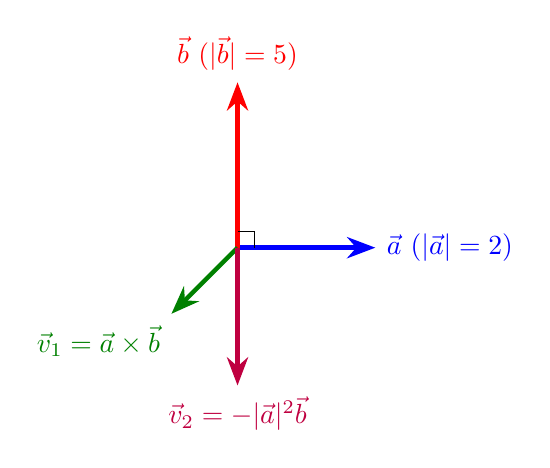
\begin{tikzpicture}[scale=0.7, >=Stealth]
  \draw[->, ultra thick, blue] (0,0) -- (2.5,0) node[right]{$\vec{a}$ ($|\vec{a}|=2$)};
  \draw[->, ultra thick, red] (0,0) -- (0,3) node[above]{$\vec{b}$ ($|\vec{b}|=5$)};
  \draw[->, ultra thick, green!50!black] (0,0) -- (-1.2,-1.2) node[below left]{$\vec{v}_1 = \vec{a} \times \vec{b}$};
  \draw[->, ultra thick, purple] (0,0) -- (0,-2.5) node[below]{$\vec{v}_2 = -|\vec{a}|^2 \vec{b}$};
  \draw (0.3,0) -- (0.3,0.3) -- (0,0.3);
\end{tikzpicture}
\end{center}

\textbf{সমাধান:} \\
ধরি, প্রথম ক্রস গুণফল $\vec{v}_1 = \vec{a} \times \vec{b}$। \\
ভেক্টর ত্রয়ী গুণফলের সূত্র $(\vec{x} \times \vec{y}) \times \vec{z} = (\vec{x} \cdot \vec{z})\vec{y} - (\vec{y} \cdot \vec{z})\vec{x}$ ব্যবহার করে পাই:
$$\vec{v}_2 = \vec{a} \times (\vec{a} \times \vec{b}) = (\vec{a} \cdot \vec{b})\vec{a} - (\vec{a} \cdot \vec{a})\vec{b}$$
যেহেতু $\vec{a} \cdot \vec{b} = 0$ এবং $\vec{a} \cdot \vec{a} = |\vec{a}|^2$:
$$\vec{v}_2 = -|\vec{a}|^2 \vec{b}$$
একইভাবে পরবর্তী ক্রস গুণফলগুলো পর্যায়ক্রমে নির্ণয় করি:
$$\vec{v}_3 = \vec{a} \times \vec{v}_2 = \vec{a} \times (-|\vec{a}|^2 \vec{b}) = -|\vec{a}|^2 (\vec{a} \times \vec{b})$$
$$\vec{v}_4 = \vec{a} \times \vec{v}_3 = \vec{a} \times \left( -|\vec{a}|^2 (\vec{a} \times \vec{b}) \right) = -|\vec{a}|^2 \left[ \vec{a} \times (\vec{a} \times \vec{b}) \right] = -|\vec{a}|^2 \left( -|\vec{a}|^2 \vec{b} \right) = |\vec{a}|^4 \vec{b}$$
$$\vec{v}_5 = \vec{a} \times \vec{v}_4 = \vec{a} \times \left( |\vec{a}|^4 \vec{b} \right) = |\vec{a}|^4 (\vec{a} \times \vec{b})$$
$$\vec{v}_6 = \vec{a} \times \vec{v}_5 = \vec{a} \times \left( |\vec{a}|^4 (\vec{a} \times \vec{b}) \right) = |\vec{a}|^4 \left[ \vec{a} \times (\vec{a} \times \vec{b}) \right] = |\vec{a}|^4 \left( -|\vec{a}|^2 \vec{b} \right) = -|\vec{a}|^6 \vec{b}$$
প্রদত্ত মান $|\vec{a}| = 2$ বসিয়ে পাই:
$$-|\vec{a}|^6 \vec{b} = -(2)^6 \vec{b} = -64\vec{b}$$
\textbf{উত্তর:} $-64\vec{b}$

\vspace{0.8cm}

% ----------------------------------------------------------------------
% Question 54
% ----------------------------------------------------------------------
\noindent\rule{\textwidth}{1pt}
\subsection*{প্রশ্ন ৫৪ (Question 54)}

\textbf{প্রশ্ন:} ধরি, একটি অজানা ভেক্টর $\vec{c} = x\hat{i} + y\hat{j} + z\hat{k}$ যা $\vec{a} = 2\hat{i} + 3\hat{j} - \hat{k}$ এবং $\vec{b} = \hat{j} + \hat{k}$ ভেক্টরদ্বয়ের সমতলে অবস্থিত (coplanar)। যদি $\vec{c}$ ভেক্টরটি $\vec{a}$ ভেক্টরের উপর লম্ব হয় এবং $\vec{c} \cdot \vec{b} = 24$ সম্পর্কটি সিদ্ধ করে, তবে $\vec{c}$ ভেক্টরটি এবং এর মান নির্ণয় করো।

(Let an unknown vector be $\vec{c} = x\hat{i} + y\hat{j} + z\hat{k}$ which is coplanar with vectors $\vec{a} = 2\hat{i} + 3\hat{j} - \hat{k}$ and $\vec{b} = \hat{j} + \hat{k}$. If $\vec{c}$ is perpendicular to $\vec{a}$ and satisfies $\vec{c} \cdot \vec{b} = 24$, find the vector $\vec{c}$ and its magnitude.)

\begin{center}
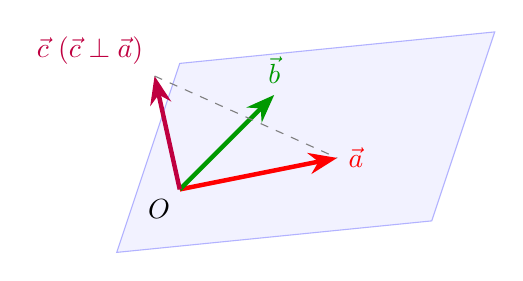
\begin{tikzpicture}[scale=0.8, >=Stealth]
  \draw[fill=blue!5, draw=blue!30] (-1,-1) -- (4,-0.5) -- (5,2.5) -- (0,2) -- cycle;
  \draw[->, ultra thick, red] (0,0) -- (2.5,0.5) node[right]{$\vec{a}$};
  \draw[->, ultra thick, green!60!black] (0,0) -- (1.5,1.5) node[above]{$\vec{b}$};
  \draw[->, ultra thick, purple] (0,0) -- (-0.4,1.8) node[above left]{$\vec{c}$ ($\vec{c} \perp \vec{a}$)};
  \draw (0,0) node[below left]{$O$};
  \draw[dashed, gray] (-0.4,1.8) -- (2.5,0.5);
\end{tikzpicture}
\end{center}

\textbf{সমাধান:} \\
১. সমতলীয় হওয়ার শর্তানুসারে (Scalar Triple Product = 0): \\
যেহেতু $\vec{c}$, $\vec{a}$ এবং $\vec{b}$ একই সমতলে অবস্থিত, তাই তাদের নির্ণায়কের মান শূন্য হতে হবে:
$$\begin{vmatrix} x & y & z \\ 2 & 3 & -1 \\ 0 & 1 & 1 \end{vmatrix} = 0$$
$$\Rightarrow x(3(1) - (-1)(1)) - y(2(1) - (-1)(0)) + z(2(1) - 3(0)) = 0$$
$$\Rightarrow x(3 + 1) - y(2) + z(2) = 0$$
$$\Rightarrow 4x - 2y + 2z = 0 \implies 2x - y + z = 0 \quad \text{--- (i)}$$
২. লম্ব হওয়ার শর্তানুসারে (Dot Product = 0): \\
যেহেতু $\vec{c}$ ভেক্টরটি $\vec{a}$ এর উপর লম্ব, তাই:
$$\vec{c} \cdot \vec{a} = 0 \implies (x\hat{i} + y\hat{j} + z\hat{k}) \cdot (2\hat{i} + 3\hat{j} - \hat{k}) = 0$$
$$\Rightarrow 2x + 3y - z = 0 \quad \text{--- (ii)}$$
৩. তৃতীয় শর্তানুসারে ($\vec{c} \cdot \vec{b} = 24$):
$$\vec{c} \cdot \vec{b} = 24 \implies (x\hat{i} + y\hat{j} + z\hat{k}) \cdot (\hat{j} + \hat{k}) = 24$$
$$\Rightarrow y + z = 24 \implies z = 24 - y \quad \text{--- (iii)}$$
সমীকরণ (i) এবং (ii) যোগ করে পাই:
$$(2x - y + z) + (2x + 3y - z) = 0 \implies 4x + 2y = 0 \implies y = -2x \quad \text{--- (iv)}$$
এখন সমীকরণ (iv) ও (iii) এর মান সমীকরণ (i)-এ বসিয়ে পাই:
$$2x - (-2x) + (24 + 2x) = 0$$
$$\Rightarrow 6x + 24 = 0 \implies 6x = -24 \implies x = -4$$
প্রাপ্ত $x$ এর মান ব্যবহার করে $y$ ও $z$ এর মান পাই:
$$y = -2(-4) = 8$$
$$z = 24 - 8 = 16$$
অতএব, নির্ণেয় ভেক্টরটি:
$$\vec{c} = -4\hat{i} + 8\hat{j} + 16\hat{k}$$
ভেক্টরের মান (Magnitude):
$$|\vec{c}| = \sqrt{(-4)^2 + 8^2 + 16^2} = \sqrt{16 + 64 + 256} = \sqrt{336} = 4\sqrt{21}$$
\textbf{উত্তর:} $\vec{c} = -4\hat{i} + 8\hat{j} + 16\hat{k}$ এবং মান $4\sqrt{21}$

\vspace{0.8cm}

% ----------------------------------------------------------------------
% Question 55
% ----------------------------------------------------------------------
\noindent\rule{\textwidth}{1pt}
\subsection*{প্রশ্ন ৫৫ (Question 55)}

\textbf{প্রশ্ন:} একটি আলোক রশ্মি $\vec{A}_{\text{in}} = -2\hat{i} - 5\hat{j}$ দিক বরাবর এসে মূলবিন্দুতে অবস্থিত একটি সমতল দর্পণ (যা x-অক্ষ বরাবর অবস্থিত) দ্বারা প্রতিফলিত হয়ে প্রতিফলিত রশ্মিটি $\vec{A}_{\text{out}}$ ভেক্টর বরাবর xy তলে গমন করে। আপতিত আলোক রশ্মি এবং প্রতিফলিত আলোক রশ্মির দিক নির্দেশকারী ভেক্টরদ্বয়ের মধ্যবর্তী কোণ ভেক্টর জ্যামিতির সাহায্যে নির্ণয় করো।

(A light ray traveling in the direction of vector $\vec{A}_{\text{in}} = -2\hat{i} - 5\hat{j}$ is reflected at the origin by a plane mirror lying along the x-axis, and the reflected ray travels along vector $\vec{A}_{\text{out}}$ in the xy-plane. Find the angle between the directional vectors of the incident light ray and the reflected light ray using vector geometry.)

\begin{center}
\begin{tikzpicture}[scale=0.6, >=Stealth]
  \fill[gray!30] (-3,0) rectangle (3,-0.2);
  \draw[thick] (-3,0) -- (3,0) node[right]{$x$-অক্ষ (দর্পণ)};
  \draw[dashed] (0,0) -- (0,3) node[above]{$\hat{n} = \hat{j}$};
  \draw[->, ultra thick, red] (-2,-4) -- (0,0) node[midway, left]{$\vec{A}_{\text{in}} = -2\hat{i}-5\hat{j}$};
  \draw[->, ultra thick, blue] (0,0) -- (-2,4) node[midway, left]{$\vec{A}_{\text{out}} = -2\hat{i}+5\hat{j}$};
  \draw[->, thick, dotted] (0,0) -- (2,4) node[right]{$-\vec{A}_{\text{in}}$};
  \draw[<->] (-0.8,1.6) arc (116:64:1.8) node[midway, above]{$\theta \approx 136.4^\circ$};
\end{tikzpicture}
\end{center}

\textbf{সমাধান:} \\
১. প্রতিফলিত ভেক্টর ($\vec{A}_{\text{out}}$) নির্ণয়: \\
সমতল দর্পণটি x-অক্ষ বরাবর অবস্থিত হওয়ায় দর্পণের অভিলম্বটি y-অক্ষের ধনাত্মক দিক বরাবর খাড়া উপরের দিকে ক্রিয়াশীল থাকবে। অতএব, একক অভিলম্ব ভেক্টর: $\hat{n} = \hat{j}$। \\
ভেক্টর প্রতিফলন সূত্রানুসারে প্রতিফলিত রশ্মির দিক নির্দেশক ভেক্টর:
$$\vec{A}_{\text{out}} = \vec{A}_{\text{in}} - 2(\vec{A}_{\text{in}} \cdot \hat{n})\hat{n}$$
এখানে ডট গুণফলের মান:
$$\vec{A}_{\text{in}} \cdot \hat{n} = (-2\hat{i} - 5\hat{j}) \cdot \hat{j} = -5$$
মানটি বসিয়ে প্রতিফলিত রশ্মির ভেক্টর পাই:
$$\vec{A}_{\text{out}} = (-2\hat{i} - 5\hat{j}) - 2(-5)\hat{j} = -2\hat{i} - 5\hat{j} + 10\hat{j} = -2\hat{i} + 5\hat{j}$$
২. ভেক্টরদ্বয়ের মধ্যবর্তী কোণ ($\theta$) নির্ণয়: \\
ধরি, আপতিত ও প্রতিফলিত ভেক্টরের মধ্যবর্তী কোণ $\theta$।
$$\cos\theta = \frac{\vec{A}_{\text{in}} \cdot \vec{A}_{\text{out}}}{|\vec{A}_{\text{in}}| |\vec{A}_{\text{out}}|}$$
এখানে:
$$\vec{A}_{\text{in}} \cdot \vec{A}_{\text{out}} = (-2\hat{i} - 5\hat{j}) \cdot (-2\hat{i} + 5\hat{j}) = (-2)(-2) + (-5)(5) = 4 - 25 = -21$$
$$|\vec{A}_{\text{in}}| = \sqrt{(-2)^2 + (-5)^2} = \sqrt{29}$$
$$|\vec{A}_{\text{out}}| = \sqrt{(-2)^2 + 5^2} = \sqrt{29}$$
অতএব:
$$\cos\theta = \frac{-21}{\sqrt{29}\sqrt{29}} = -\frac{21}{29}$$
$$\Rightarrow \theta = \cos^{-1}\left( -\frac{21}{29} \right) \approx 136.4^\circ$$
\textbf{উত্তর:} আপতিত ও প্রতিফলিত রশ্মির মধ্যবর্তী কোণ $\approx 136.4^\circ$

\vspace{0.8cm}

% ----------------------------------------------------------------------
% Question 56
% ----------------------------------------------------------------------
\noindent\rule{\textwidth}{1pt}
\subsection*{প্রশ্ন ৫৬ (Question 56)}

\textbf{প্রশ্ন:} যদি $\vec{A}$, $\vec{B}$ এবং $\vec{C}$ তিনটি এমন ভেক্টর হয় যেন $|\vec{B}| = |\vec{C}|$। ভেক্টর বীজগণিতের সূত্রাবলি ব্যবহার করে প্রমাণ করো যে, $[(\vec{A}+\vec{B}) \times (\vec{A}+\vec{C})] \times (\vec{B} \times \vec{C}) \cdot (\vec{B}+\vec{C}) = 0$।

(If $\vec{A}$, $\vec{B}$, and $\vec{C}$ are three vectors such that $|\vec{B}| = |\vec{C}|$, prove using vector algebra that $[(\vec{A}+\vec{B}) \times (\vec{A}+\vec{C})] \times (\vec{B} \times \vec{C}) \cdot (\vec{B}+\vec{C}) = 0$.)

\begin{center}
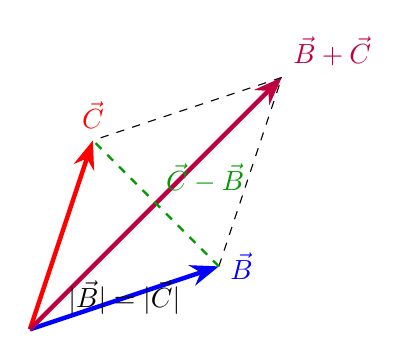
\begin{tikzpicture}[scale=0.8, >=Stealth]
  \coordinate (O) at (0,0);
  \draw[->, ultra thick, blue] (O) -- (3,1) node[right]{$\vec{B}$};
  \draw[->, ultra thick, red] (O) -- (1,3) node[above]{$\vec{C}$};
  \draw[->, ultra thick, purple] (O) -- (4,4) node[above right]{$\vec{B}+\vec{C}$};
  \draw[dashed] (3,1) -- (4,4) -- (1,3);
  \draw[dashed, green!60!black, thick] (3,1) -- (1,3) node[midway, above right]{$\vec{C}-\vec{B}$};
  \node at (1.5,0.5) {$|\vec{B}| = |\vec{C}|$};
\end{tikzpicture}
\end{center}

\textbf{সমাধান:} \\
ধরি, $\vec{u} = (\vec{A}+\vec{B}) \times (\vec{A}+\vec{C})$। \\
বণ্টন সূত্র প্রয়োগ করে পাই:
$$\vec{u} = \vec{A} \times \vec{A} + \vec{A} \times \vec{C} + \vec{B} \times \vec{A} + \vec{B} \times \vec{C}$$
যেহেতু $\vec{A} \times \vec{A} = \vec{0}$ এবং $\vec{B} \times \vec{A} = - \vec{A} \times \vec{B}$:
$$\vec{u} = \vec{A} \times \vec{C} - \vec{A} \times \vec{B} + \vec{B} \times \vec{C} = \vec{A} \times (\vec{C} - \vec{B}) + \vec{B} \times \vec{C} \quad \text{--- (i)}$$
এখন ভেক্টর ত্রয়ী গুণফলের সূত্র $(\vec{x} \times \vec{y}) \times \vec{z} = (\vec{x} \cdot \vec{z})\vec{y} - (\vec{y} \cdot \vec{z})\vec{x}$ ব্যবহার করে পাই:
$$\vec{u} \times (\vec{B} \times \vec{C}) = (\vec{u} \cdot \vec{C})\vec{B} - (\vec{u} \cdot \vec{B})\vec{C}$$
এবার এই ভেক্টরটিকে $(\vec{B}+\vec{C})$ এর সাথে ডট গুণ করি:
$$\text{LHS} = \left[ (\vec{u} \cdot \vec{C})\vec{B} - (\vec{u} \cdot \vec{B})\vec{C} \right] \cdot (\vec{B}+\vec{C})$$
$$\Rightarrow \text{LHS} = (\vec{u} \cdot \vec{C})|\vec{B}|^2 + (\vec{u} \cdot \vec{C})(\vec{B} \cdot \vec{C}) - (\vec{u} \cdot \vec{B})(\vec{C} \cdot \vec{B}) - (\vec{u} \cdot \vec{B})|\vec{C}|^2$$
ধরি, $|\vec{B}|^2 = |\vec{C}|^2 = b^2$ এবং $\vec{B} \cdot \vec{C} = k$।
$$\text{LHS} = (\vec{u} \cdot \vec{C})b^2 + (\vec{u} \cdot \vec{C})k - (\vec{u} \cdot \vec{B})k - (\vec{u} \cdot \vec{B})b^2$$
$$\Rightarrow \text{LHS} = \left[ \vec{u} \cdot (\vec{C} - \vec{B}) \right] (b^2 + k) \quad \text{--- (ii)}$$
এখন সমীকরণ (i) থেকে প্রাপ্ত $\vec{u}$ এর মান সমীকরণ (ii)-এর $\vec{u} \cdot (\vec{C} - \vec{B})$ অংশে বসিয়ে পাই:
$$\vec{u} \cdot (\vec{C} - \vec{B}) = \left[ \vec{A} \times (\vec{C} - \vec{B}) + \vec{B} \times \vec{C} \right] \cdot (\vec{C} - \vec{B})$$
$$\Rightarrow \vec{u} \cdot (\vec{C} - \vec{B}) = \underbrace{[\vec{A} \times (\vec{C} - \vec{B})] \cdot (\vec{C} - \vec{B})}_{=0} + \underbrace{(\vec{B} \times \vec{C}) \cdot (\vec{C} - \vec{B})}_{=0}$$
$$\Rightarrow \vec{u} \cdot (\vec{C} - \vec{B}) = 0$$
যেহেতু $\vec{u} \cdot (\vec{C} - \vec{B}) = 0$, সেহেতু সমীকরণ (ii) থেকে পাই:
$$\text{LHS} = 0 \times (b^2 + k) = 0 \quad \text{(প্রমাণিত)}$$

\vspace{0.8cm}

% ----------------------------------------------------------------------
% Question 57
% ----------------------------------------------------------------------
\noindent\rule{\textwidth}{1pt}
\subsection*{প্রশ্ন ৫৭ (Question 57)}

\textbf{প্রশ্ন:} ত্রিমাত্রিক স্থানে যেকোনো দুটি ভেক্টর $\vec{u}$ এবং $\vec{v}$ এর জন্য ভেক্টর বীজগণিতের মৌলিক সূত্রাবলি ও ল্যাগরঞ্জের অভেদ ব্যবহার করে প্রমাণ করো যে, $(1 + |\vec{u}|^2)(1 + |\vec{v}|^2) = (1 - \vec{u} \cdot \vec{v})^2 + |\vec{u} + \vec{v} + (\vec{u} \times \vec{v})|^2$।

(For any two vectors $\vec{u}$ and $\vec{v}$ in 3D space, prove using fundamental rules of vector algebra and Lagrange's identity that $(1 + |\vec{u}|^2)(1 + |\vec{v}|^2) = (1 - \vec{u} \cdot \vec{v})^2 + |\vec{u} + \vec{v} + (\vec{u} \times \vec{v})|^2$.)

\begin{center}
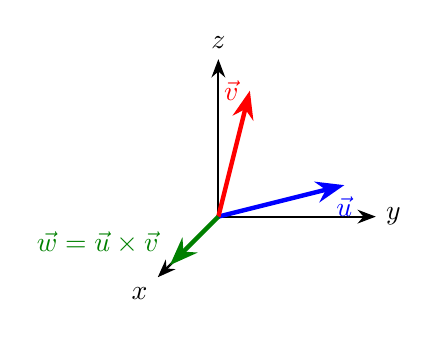
\begin{tikzpicture}[scale=0.8, >=Stealth]
  \draw[->, thick] (0,0,0) -- (2.5,0,0) node[right]{$y$};
  \draw[->, thick] (0,0,0) -- (0,2.5,0) node[above]{$z$};
  \draw[->, thick] (0,0,0) -- (0,0,2.5) node[below left]{$x$};
  \draw[->, ultra thick, blue] (0,0,0) -- (2,0.5,0) node[below]{$\vec{u}$};
  \draw[->, ultra thick, red] (0,0,0) -- (0.5,2,0) node[left]{$\vec{v}$};
  \draw[->, ultra thick, green!50!black] (0,0,0) -- (0,0,2) node[above left]{$\vec{w} = \vec{u}\times\vec{v}$};
\end{tikzpicture}
\end{center}

\textbf{সমাধান:} \\
প্রথমে বামপক্ষ (LHS) বিস্তৃত করি:
$$\text{LHS} = (1 + |\vec{u}|^2)(1 + |\vec{v}|^2) = 1 + |\vec{u}|^2 + |\vec{v}|^2 + |\vec{u}|^2 |\vec{v}|^2 \quad \text{--- (i)}$$
এবার ডানপক্ষ (RHS) দুটি আলাদা অংশে বিস্তৃত করি: \\
১ম অংশ:
$$\text{Part}_1 = (1 - \vec{u} \cdot \vec{v})^2 = 1 - 2(\vec{u} \cdot \vec{v}) + (\vec{u} \cdot \vec{v})^2$$
২য় অংশ (ধরি $\vec{w} = \vec{u} \times \vec{v}$):
$$\text{Part}_2 = |\vec{u} + \vec{v} + \vec{w}|^2 = (\vec{u} + \vec{v} + \vec{w}) \cdot (\vec{u} + \vec{v} + \vec{w})$$
$$\Rightarrow \text{Part}_2 = |\vec{u}|^2 + |\vec{v}|^2 + |\vec{w}|^2 + 2(\vec{u} \cdot \vec{v}) + 2(\vec{u} \cdot \vec{w}) + 2(\vec{v} \cdot \vec{w})$$
যেহেতু $\vec{w} = \vec{u} \times \vec{v}$ ভেক্টরটি $\vec{u}$ এবং $\vec{v}$ উভয়ের উপর লম্ব, তাই তাদের ডট গুণফল শূন্য হবে:
$$\vec{u} \cdot \vec{w} = 0 \quad \text{এবং} \quad \vec{v} \cdot \vec{w} = 0$$
অতএব:
$$\text{Part}_2 = |\vec{u}|^2 + |\vec{v}|^2 + |\vec{u} \times \vec{v}|^2 + 2(\vec{u} \cdot \vec{v})$$
এখন ডানপক্ষের দুটি অংশ যোগ করি:
$$\text{RHS} = \text{Part}_1 + \text{Part}_2$$
$$\Rightarrow \text{RHS} = [1 - 2(\vec{u} \cdot \vec{v}) + (\vec{u} \cdot \vec{v})^2] + [|\vec{u}|^2 + |\vec{v}|^2 + |\vec{u} \times \vec{v}|^2 + 2(\vec{u} \cdot \vec{v})]$$
$$\Rightarrow \text{RHS} = 1 + |\vec{u}|^2 + |\vec{v}|^2 + \left[ (\vec{u} \cdot \vec{v})^2 + |\vec{u} \times \vec{v}|^2 \right]$$
ল্যাগরঞ্জের অভেদ (Lagrange's Identity) $(\vec{u} \cdot \vec{v})^2 + |\vec{u} \times \vec{v}|^2 = |\vec{u}|^2 |\vec{v}|^2$ প্রয়োগ করে পাই:
$$\text{RHS} = 1 + |\vec{u}|^2 + |\vec{v}|^2 + |\vec{u}|^2 |\vec{v}|^2$$
সমীকরণ (i) এবং এই প্রাপ্ত ফলাফল তুলনা করে দেখা যাচ্ছে:
$$\text{LHS} = \text{RHS} \quad \text{(প্রমাণিত)}$$

\vspace{0.8cm}

% ----------------------------------------------------------------------
% Question 58
% ----------------------------------------------------------------------
\noindent\rule{\textwidth}{1pt}
\subsection*{প্রশ্ন ৫৮ (Question 58)}

\textbf{প্রশ্ন:} ধরি, $\vec{a}$, $\vec{b}$ এবং $\vec{c}$ তিনটি অসমতলীয় (non-coplanar) একক ভেক্টর, যারা পরস্পরের সাথে সমান কোণ $\theta$ উৎপন্ন করে। যদি $\vec{a} \times \vec{b} + \vec{b} \times \vec{c} = p\vec{a} + q\vec{b} + r\vec{c}$ হয়, তবে স্কেলার ধ্রুবক $p$, $q$ এবং $r$ এর মান $\theta$ এর মাধ্যমে প্রকাশ করো।

(Let $\vec{a}$, $\vec{b}$, and $\vec{c}$ be three non-coplanar unit vectors mutually inclined at equal angle $\theta$. If $\vec{a} \times \vec{b} + \vec{b} \times \vec{c} = p\vec{a} + q\vec{b} + r\vec{c}$, express the scalar constants $p$, $q$, and $r$ in terms of $\theta$.)

\begin{center}
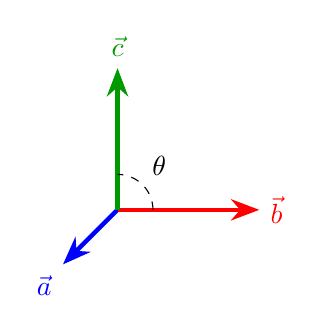
\begin{tikzpicture}[scale=0.9, >=Stealth]
  \draw[->, ultra thick, blue] (0,0,0) -- (0,0,2) node[below left]{$\vec{a}$};
  \draw[->, ultra thick, red] (0,0,0) -- (2,0,0) node[right]{$\vec{b}$};
  \draw[->, ultra thick, green!60!black] (0,0,0) -- (0,2,0) node[above]{$\vec{c}$};
  \draw[dashed] (0.5,0,0) arc (0:90:0.5) node[midway, above right]{$\theta$};
\end{tikzpicture}
\end{center}

\textbf{সমাধান:} \\
দেওয়া আছে, $|\vec{a}| = |\vec{b}| = |\vec{c}| = 1$ এবং $\vec{a} \cdot \vec{b} = \vec{b} \cdot \vec{c} = \vec{c} \cdot \vec{a} = \cos\theta$। \\
প্রদত্ত সমীকরণটির উভয় পক্ষে যথাক্রমে $\vec{a}$, $\vec{b}$ এবং $\vec{c}$ দ্বারা ডট গুণ করে তিনটি সমীকরণ তৈরি করি: \\
১. $\vec{a}$ দ্বারা ডট গুণ করে পাই (যেহেতু $\vec{a} \cdot (\vec{a} \times \vec{b}) = 0$):
$$[\vec{a} \ \vec{b} \ \vec{c}] = p + (q+r)\cos\theta \quad \text{--- (i)}$$
২. $\vec{b}$ দ্বারা ডট গুণ করে পাই:
$$0 = p\cos\theta + q + r\cos\theta \implies q = -(p+r)\cos\theta \quad \text{--- (ii)}$$
৩. $\vec{c}$ দ্বারা ডট গুণ করে পাই (যেহেতু $\vec{c} \cdot (\vec{b} \times \vec{c}) = 0$):
$$[\vec{a} \ \vec{b} \ \vec{c}] = (p+q)\cos\theta + r \quad \text{--- (iii)}$$
সমীকরণ (i) এবং (iii) তুলনা করে পাই:
$$p + (q+r)\cos\theta = r + (p+q)\cos\theta \implies p(1-\cos\theta) = r(1-\cos\theta)$$
যেহেতু ভেক্টর তিনটি অসমতলীয়, তাই $\theta \neq 0$ এবং $\cos\theta \neq 1$। অতএব:
$$p = r \quad \text{--- (iv)}$$
সমীকরণ (iv) এর মান সমীকরণ (ii)-এ বসিয়ে পাই:
$$q = -2p\cos\theta \quad \text{--- (v)}$$
সমান কোণে আনত তিনটি একক ভেক্টরের স্কেলার ত্রয়ী গুণফল ও কোণের সম্পর্কটি হলো:
$$[\vec{a} \ \vec{b} \ \vec{c}] = (1-\cos\theta)\sqrt{1+2\cos\theta} \quad \text{--- (vi)}$$
এখন সমীকরণ (v) ও (iv)-এর মান সমীকরণ (i)-এ বসিয়ে পাই:
$$[\vec{a} \ \vec{b} \ \vec{c}] = p + (-2p\cos\theta + p)\cos\theta = p(1+\cos\theta-2\cos^2\theta) = p(1-\cos\theta)(1+2\cos\theta)$$
সমীকরণ (vi) থেকে সমাধান করে পাই:
$$(1-\cos\theta)\sqrt{1+2\cos\theta} = p(1-\cos\theta)(1+2\cos\theta)$$
$$\Rightarrow p = \frac{\sqrt{1+2\cos\theta}}{1+2\cos\theta} = \frac{1}{\sqrt{1+2\cos\theta}}$$
\textbf{উত্তর:} $p = r = \frac{1}{\sqrt{1+2\cos\theta}}, \quad q = \frac{-2\cos\theta}{\sqrt{1+2\cos\theta}}$

\vspace{0.8cm}

% ----------------------------------------------------------------------
% Question 59
% ----------------------------------------------------------------------
\noindent\rule{\textwidth}{1pt}
\subsection*{প্রশ্ন ৫৯ (Question 59)}

\textbf{প্রশ্ন:} অবস্থান ভেক্টর $\vec{r} = x\hat{i} + y\hat{j} + z\hat{k}$ এবং $r = |\vec{r}|$ হলে, ভেক্টর ক্যালকুলাসের অপারেটর ও অন্তরীকরণের গুণন সূত্র প্রয়োগ করে প্রমাণ করো যে, $\vec{\nabla} \cdot (r^n \vec{r}) = (n+3)r^n$। এর সাহায্যে $\vec{\nabla} \cdot (r^3 \vec{r})$ এবং $\vec{\nabla} \cdot \left(\frac{\vec{r}}{r^3}\right)$ এর মান নির্ণয় করো।

(Given position vector $\vec{r} = x\hat{i} + y\hat{j} + z\hat{k}$ and $r = |\vec{r}|$, use vector calculus operators and differentiation product rules to prove that $\vec{\nabla} \cdot (r^n \vec{r}) = (n+3)r^n$. Using this, evaluate $\vec{\nabla} \cdot (r^3 \vec{r})$ and $\vec{\nabla} \cdot \left(\frac{\vec{r}}{r^3}\right)$.)

\begin{center}
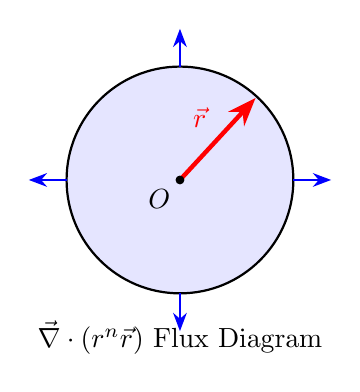
\begin{tikzpicture}[scale=0.8, >=Stealth]
  \draw[thick, fill=blue!10] (0,0) circle (1.8);
  \draw[->, ultra thick, red] (0,0) -- (1.2,1.3) node[midway, above left]{$\vec{r}$};
  \fill (0,0) circle (2pt) node[below left]{$O$};
  \draw[->, thick, blue] (1.8,0) -- (2.4,0);
  \draw[->, thick, blue] (-1.8,0) -- (-2.4,0);
  \draw[->, thick, blue] (0,1.8) -- (0,2.4);
  \draw[->, thick, blue] (0,-1.8) -- (0,-2.4);
  \node at (0,-2.5) {$\vec{\nabla}\cdot(r^n\vec{r})$ Flux Diagram};
\end{tikzpicture}
\end{center}

\textbf{সমাধান:} \\
আমরা জানি, ভেক্টর ক্যালকুলাসের ডাইভারজেন্স গুণন সূত্র (Divergence product rule):
$$\vec{\nabla} \cdot (\phi \vec{A}) = \phi(\vec{\nabla} \cdot \vec{A}) + \vec{A} \cdot (\vec{\nabla}\phi)$$
এখানে $\phi = r^n$ এবং $\vec{A} = \vec{r}$ ধরি:
$$\vec{\nabla} \cdot (r^n \vec{r}) = r^n(\vec{\nabla} \cdot \vec{r}) + \vec{r} \cdot (\vec{\nabla}r^n) \quad \text{--- (i)}$$
আমরা জানি: \\
১. $\vec{\nabla} \cdot \vec{r} = \frac{\partial x}{\partial x} + \frac{\partial y}{\partial y} + \frac{\partial z}{\partial z} = 1 + 1 + 1 = 3$ \\
২. $\vec{\nabla}r^n = n r^{n-2} \vec{r}$ (গ্রেডিয়েন্টের সাধারণ সূত্র থেকে)

এই মানগুলো সমীকরণ (i)-এ বসিয়ে পাই:
$$\vec{\nabla} \cdot (r^n \vec{r}) = r^n(3) + \vec{r} \cdot (n r^{n-2} \vec{r}) = 3r^n + n r^{n-2}(\vec{r} \cdot \vec{r})$$
যেহেতু $\vec{r} \cdot \vec{r} = r^2$:
$$\vec{\nabla} \cdot (r^n \vec{r}) = 3r^n + n r^{n-2}(r^2) = 3r^n + n r^n = (n+3)r^n \quad \text{(প্রমাণিত)}$$

\textbf{প্রয়োগসমূহ:} \\
১ম ক্ষেত্র ($n=3$):
$$\vec{\nabla} \cdot (r^3 \vec{r}) = (3+3)r^3 = 6r^3$$
২য় ক্ষেত্র ($n=-3$):
$$\vec{\nabla} \cdot \left(\frac{\vec{r}}{r^3}\right) = \vec{\nabla} \cdot (r^{-3} \vec{r}) = (-3+3)r^{-3} = 0$$
\textbf{উত্তর:} ১ম ক্ষেত্রে $6r^3$ এবং ২য় ক্ষেত্রে $0$

\vspace{0.8cm}

% ----------------------------------------------------------------------
% Question 60
% ----------------------------------------------------------------------
\noindent\rule{\textwidth}{1pt}
\subsection*{প্রশ্ন ৬০ (Question 60)}

\textbf{প্রশ্ন:} একটি স্রোতস্বিনী নদীতে নৌকার বেগ $2\text{ m/s}$ হলে তা ন্যূনতম দূরত্ব বা সোজা পথে অপর পাড়ে পৌঁছাতে পারে। এতে যে সময় লাগে, নদীতে স্রোত না থাকলে নৌকাটি দিয়ে সর্বনিম্ন সময়ে পার হতে তার ঠিক অর্ধেক সময় লাগত। স্রোতের বেগ কত? নদীর প্রস্থ $100\text{ m}$ হলে নৌকাটির পক্ষে নদী পারাপার হতে ন্যূনতম কত সময় লাগবে?

(If the speed of a boat in a flowing river is $2\text{ m/s}$, it can cross to the opposite bank along the shortest path. The time required for this is twice the minimum time required to cross the river when there is no current. What is the speed of the current? If the river width is $100\text{ m}$, what is the minimum time required for the boat to cross the river?)

\begin{center}
\begin{tikzpicture}[scale=0.8, >=Stealth]
  \draw[ultra thick, blue] (-1,0) -- (5,0) node[right]{নদীর তীর ১};
  \draw[ultra thick, blue] (-1,3) -- (5,3) node[right]{নদীর তীর ২};
  \draw[->, thick, cyan] (0,0.4) -- (1,0.4) node[right]{স্রোতের বেগ $u$};
  \draw[->, thick, cyan] (2.5,0.4) -- (3.5,0.4);
  \draw[->, ultra thick, red] (0,0) -- (0,3) node[midway, right]{$w = \sqrt{v^2-u^2}$};
  \draw[->, ultra thick, green!60!black] (0,0) -- (-1.732,3) node[midway, left]{$v=2\text{ m/s}$};
  \draw[->, ultra thick, cyan] (-1.732,3) -- (0,3) node[midway, above]{$u$};
  \draw[dashed] (0,0) -- (0,3);
  \node at (3.5,1.5) {$d = 100\text{ m}$};
\end{tikzpicture}
\end{center}

\textbf{সমাধান:} \\
ধরি, নৌকার বেগ $v = 2\text{ m/s}$, স্রোতের বেগ $= u$, এবং নদীর প্রস্থ $d = 100\text{ m}$।

\textbf{১ম ক্ষেত্রে (ন্যূনতম পথে নদী পার হতে সময় $t_1$):} \\
সোজা বিপরীত পাড়ে পৌঁছানোর জন্য কার্যকরী বেগ $w = \sqrt{v^2-u^2}$।
$$t_1 = \frac{d}{\sqrt{v^2-u^2}} \quad \text{--- (i)}$$

\textbf{২য় ক্ষেত্রে (স্রোতহীন নদীতে সর্বনিম্ন সময়ে পারাপার হতে সময় $t_2$):} \\
স্রোত না থাকলে সরাসরি সোজা রওনা দিলে সবচেয়ে কম সময় লাগবে।
$$t_2 = \frac{d}{v} \quad \text{--- (ii)}$$

\textbf{শর্তানুসারে:}
$$t_2 = \frac{1}{2}t_1 \implies \frac{d}{v} = \frac{d}{2\sqrt{v^2-u^2}}$$
$$\Rightarrow 2\sqrt{v^2-u^2} = v$$
উভয় পক্ষকে বর্গ করে পাই:
$$4(v^2-u^2) = v^2 \implies 4v^2 - 4u^2 = v^2 \implies 3v^2 = 4u^2$$
$$\Rightarrow u = \frac{\sqrt{3}}{2}v$$
দেওয়া আছে নৌকার বেগ $v = 2\text{ m/s}$। মানটি বসিয়ে পাই:
$$u = \frac{\sqrt{3}}{2} \times 2 = \sqrt{3}\text{ m/s} \approx 1.732\text{ m/s}$$

\textbf{ন্যূনতম সময়ে নদী পারাপার ($t_{\text{min}}$):} \\
আমরা জানি, যেকোনো নদীতে সর্বনিম্ন সময়ে পার হওয়ার শর্ত হলো স্রোতের লম্ব অভিমুখে রওনা দেওয়া ($\alpha = 90^\circ$)।
$$t_{\text{min}} = \frac{d}{v} = \frac{100\text{ m}}{2\text{ m/s}} = 50\text{ s}$$
\textbf{উত্তর:} স্রোতের বেগ $\sqrt{3}\text{ m/s}$ এবং নদী পারাপারের সর্বনিম্ন সময় $50\text{ s}$

\end{document}